\documentclass[preview]{standalone}
\usepackage{tikz}
\usetikzlibrary{calc}

\begin{document}
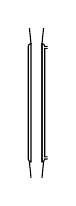
\begin{tikzpicture}
	\pgfmathsetmacro{\R}{0.5}				%radius of flask
	\pgfmathsetmacro{\width}{14}			%width of inner condenser
	\pgfmathsetmacro{\length}{150}			%length of condenser
	\pgfmathsetmacro{\pos}{90}
	\pgfmathsetmacro{\ang}{45}			%separation of necks in degrees
	\pgfmathsetmacro{\taperlength}{20}	%Length of the joint taper
	\pgfmathsetmacro{\direction}{1}
	%calculated
	\pgfmathsetmacro{\firstangle}{\pos-\ang}	%Calculating the far right angle
	\pgfmathsetmacro{\secondangle}{\pos+\ang}	%Calculating the far left angle
	\pgfmathsetmacro{\width}{\width/100}	
	\pgfmathsetmacro{\length}{\length/100}	
	\pgfmathsetmacro{\waterwidth}{0.25*\width}
	\pgfmathsetmacro{\taperwidth}{\width}	%Width of the joint taper
	\pgfmathsetmacro{\taperlength}{\taperlength/100}
	\pgfmathsetmacro{\R}{\R+\taperlength}	
	
	\coordinate (a) at (\direction*\width/2,\R+\length) {};
	\coordinate (b) at (\direction*\width/2,\R) {};
	\coordinate (c) at (\direction*-\width/2,\R) {};
	\coordinate (d) at (\direction*-\width/2,\R+\length) {};
	\coordinate (e) at (\direction*\width/2,\R+\length-\waterwidth) {};
	\coordinate (f) at (\direction*\width/2,\R+\length+\waterwidth) {};
	\coordinate (g) at (\direction*-\width/2,\R+\length+\waterwidth) {};
	\coordinate (h) at (\direction*\width/2,\R+\length-\waterwidth) {};

	%condenser
	\draw (b) -- (a) arc (90:0:\waterwidth) -- ++(\waterwidth, 0) ++ (0, -0.75*\waterwidth) -- ++(-\waterwidth, 0) -- ++(0, -{\length+3.5*\waterwidth}) -- ++(\waterwidth, 0);
	\draw (a) -- (b) arc (270:360:\waterwidth) -- ++(\waterwidth,0); 
	\draw (d) -- (c) arc (270:180:\waterwidth) -- ++(0,\length-2*\waterwidth) arc (180:90:\waterwidth) -- (c);

	%connections
	\pgfmathsetmacro{\S}{\R}	
	\coordinate (i) at ({\pos-atan((\taperwidth/2)/\S)}:\S+\taperlength) {};
	\coordinate (j) at ({\pos-atan((\taperwidth/2)/\S)}:\S) {};
	\coordinate (k) at ({\pos+atan((\taperwidth/2)/\S)}:\S) {};
	\coordinate (l) at ({\pos+atan((\taperwidth/2)/\S)}:\S+\taperlength) {};
	\draw (a) -- ($(i)+(0,\length)$) -- ($(j)+(0,\length)$);
	\draw (d) -- ($(k)+(0,\length)$) -- ($(l)+(0,\length)$);
	\draw (c) -- ($(l)+(0,-\taperlength)$) -- ($(k)+(0,-\taperlength)$);
	\draw (b) -- ($(i)+(0,-\taperlength)$) -- ($(j)+(0,-\taperlength)$);

\end{tikzpicture}
\end{document}

